\documentclass[10pt]{article}
\usepackage[a4paper,margin=16mm]{geometry}
\usepackage{mathptmx,graphicx,booktabs,hyperref}
\setlength{\parindent}{0pt}\setlength{\parskip}{5pt}\emergencystretch=2em
\begin{document}
\begin{center}{\Large Uniform useful-yield auditor: compile-only progress}\\[4pt]
Existing PR2381;26 October2026\end{center}
\textbf{No scientific execution.} The independent Rust auditor and a versioned
C++ producer now compile. The study inputs, matrix/state computations,
corruption paths and new proof statements have not run. This advances the
implementation while preserving the pending checkpoint-upload restriction.

\section*{What the implementation adds}
The fixed protocol covers all size-two/three bases on the existing F43/F13
fixtures:96arms,896 separate source targets and210uniform policy pairs are
planned. Existing actual source-DLP reductions stay pinned. The older
\texttt{uniform-yield.cpp} and its sealed preflight hashes remain unchanged.
The new version adds explicit source/twist nondominated sets over useful-rank
mean, named degree and expected collection calls, retaining every policy.

The Rust implementation uses its separately implemented field/group/polynomial
arithmetic, batch witness checks and full response reconstruction. Its own
arbitrary-precision rational normalization and breadth-first state closure,
then descending-rank solution, differ from the C++ recursive GMP path. Code
covers exact case membership, point/sign/root/solver/log/scalar fields,
state transitions/rationals, manifest/source checks and rehashed corruption
modes. These are intended checks, not executed verification results.

\begin{center}\begin{tabular}{l l}\toprule
Check & Actual outcome\\\midrule
C++ producer v2 compile/link &PASS; binary not executed\\
Rust ordinary release build &PASS; audit path not executed\\
Rust backend test-harness build &PASS with --no-run; tests not executed\\
Uniform study / replay / corruption controls &NOT RUN\\
New Lean recurrence proof / exact runner &NOT IMPLEMENTED\\\bottomrule
\end{tabular}\end{center}
\begin{center}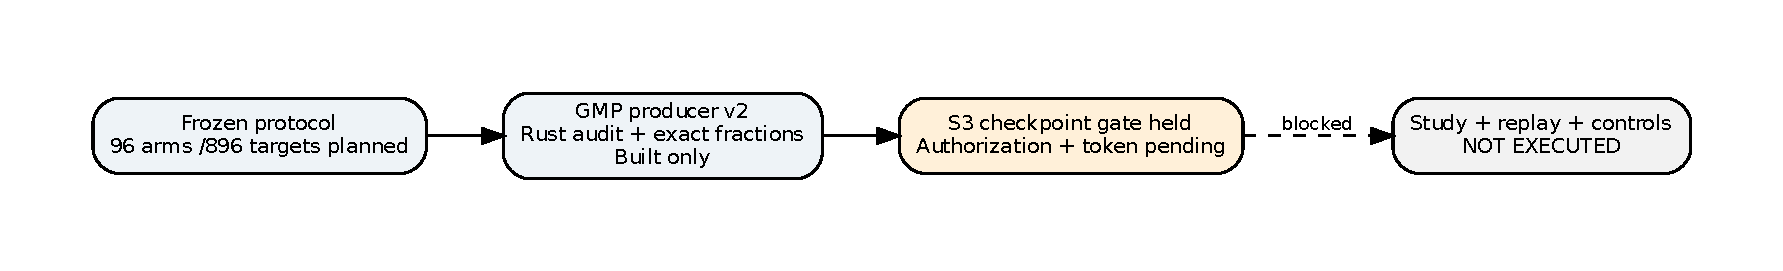
\includegraphics[width=\linewidth]{bridge.pdf}\end{center}
No mathematical result, expectation, speedup, intrinsic regularity or general
hardness claim follows from compilation. Existing208public/269audited study
declarations and17identity records remain historical and unchanged. Ordinary
unchanged root-library and metadata validation is recorded separately.

\section*{Newly exposed merge requirements}
At the parent head60b006333c9fcfa50ccf9251424a7ef0431973ac,
the active branch-rules endpoint lists three required status contexts:
\texttt{gate},\texttt{size},\texttt{artifacts}. None appears in that complete
exact-head check/status response; the sole queued review is not one of them.
No submitted review or thread exists. Legacy branch-protection access still
returns403, so other protections cannot be ruled out. The PR remains open,
non-draft and conflicted; no missing or queued check is counted as passed.
This is a newly verified gate, not a CI failure to patch around.

\section*{Authorization and the next scientific step}
Current main still requires a successful S3 resume checkpoint before experiments.
Its gate auto-uploads after a complete resume note. The user's no-extra-upload
instruction remains in force; the approval question is still pending and no
checkpoint token is configured. No gate invocation, skip, fake last-push,
upload, credential reuse or paid resource occurs in this iteration.

The next dependent step is explicit checkpoint-only authorization and secure
token setup, then the unmodified gate, faithful recurrence proof and exact
runner, followed by the complete bounded study and independent controls.
Default native cap600s and focused iteration3600s stay fixed. All prior frozen
science, registry/catalog/benchmark and conflicted files remain unchanged.
The existing single automation continues the PR follow-up; no second writer.
\end{document}
